\documentclass[conference]{IEEEtran}
\IEEEoverridecommandlockouts
% The preceding line is only needed to identify funding in the first footnote. If that is unneeded, please comment it out.
\usepackage[T1]{fontenc}
\usepackage{cite}
\usepackage{mathtools} 
\usepackage{stackengine}
\def\delequal{\mathrel{\ensurestackMath{\stackon[1pt]{=}{\scriptstyle\Delta}}}}
\usepackage{amsmath,amssymb,amsfonts}
\usepackage{amsmath,epsfig,cite,amsfonts,amssymb,psfrag,subfig}
\usepackage{graphicx}
\usepackage{textcomp}
\usepackage{xcolor}
\usepackage{algorithm}
\usepackage[noend]{algpseudocode}
\usepackage{amsthm}
\def\BibTeX{{\rm B\kern-.05em{\sc i\kern-.025em b}\kern-.08em
    T\kern-.1667em\lower.7ex\hbox{E}\kern-.125emX}}
\allowdisplaybreaks
\newtheorem{remark}{Remark}
\newtheorem{theorem}{Theorem}
\newtheorem{lemma}{Lemma}
\newtheorem{proposition}{Proposition}
\newtheorem{corollary}{Corollary}   

\begin{document}

\title{Joint Power Allocation and Network Slicing In an End to End O-RAN System
}

\author{\IEEEauthorblockN{1\textsuperscript{st} Mojdeh Karbalaee Motalleb}
\IEEEauthorblockA{\textit{Electrical and Computer Engineering} \\
\textit{Tehran University}\\
Tehran, Iran \\
mojdeh.karbalaee@ut.ac.ir}
\and
\IEEEauthorblockN{2\textsuperscript{nd} Vahid Shah-Mansouri}
\IEEEauthorblockA{\textit{Electrical and Computer Engineering} \\
\textit{Tehran University}\\
Tehran, Iran \\
vmansouri@ut.ac.ir}
\and
\IEEEauthorblockN{3\textsuperscript{rd} Salar Nouri Naghadeh}
\IEEEauthorblockA{\textit{Electrical and Computer Engineering} \\
\textit{Tehran University}\\
Tehran, Iran \\
salar.nouri@ut.ac.ir}

}

\maketitle

\begin{abstract}
Many major telecommunication companies confirmed the unification of the xRAN Group with the C-RAN Alliance to establish a more flexible and openness radio access network which is the Open-RAN 
(O-RAN) for the fifth generation of wireless technology. 


To increase enrgy efficiency and optimize the allocation of resources, Network Slicing (NS) is considered as the best method for the fifth generation (5G) in order to virtualize the common physical network into several logical end-to-end networks. Every slice consists of a part of core network resources, network functions, and radio access network resources as a functional end-to-end network. 


In this paper, we elaborate joint NS in RAN and Core of O-RAN system to investigate the power 
of each User Equipment (UE), connect slices to services and also connect physical Data Centers (DC) to slices to jointly maximize energy efficiency and minimize consumption power of RRHs and the cost of  physical resources in a downlink channel. The problem is formulated as a mixed-integer optimization problem that can be decomposed into two independent sub-problems due to the fact that sub-problems are independent. 
Heuristic algorithms are proposed to each of sub-problems in order to connect slices to services, optimize power consumption and connect slices to physical resources to minimize the cost of total DCs simultaneously.
\end{abstract}

\begin{IEEEkeywords}
O-RAN, Network Slicing, Energy Efficiency, Data Center (DC)
\end{IEEEkeywords}

\section{Introduction}
Recently, O-RAN, which is the integration and expansion of C-RAN and xRAN, is expected to be a key technology for 5G to enhance RAN performance and solve the part of challenges of mobile network operators (MNOs) in the best way.  
The Idea of O-RAN comes from two opinions. Firstly, according to real-time analytic used for artificial intelligence systems, the radio access networks must be evolved to be more intelligent and flexible than before. Furthermore, O-RAN can virtualize elements of the network with  appropriate interfaces \cite{orant}.
In an innovative O-RAN system, the programmable RAN software is decoupled from hardware, which can be run on any specific processing platforms, in order to be more flexible for MNOs especially for mobile virtual network operators (MVNOs)\cite{oran1}. 


The core idea of C-RAN is to split the radio remote head (RRH) from baseband unit (BBU). Several BBUs operating on a cloud server will create a BBU-Pool, providing unified baseband signal processing with powerful computing capabilities. Moreover, in O-RAN technology, this separation is implemented\cite{cran1}.
To communicate between BBU-Pool and RRHs, the fronthaul fiber link interface, is assumed with limited capacity. The compression of a message passed through these links is a consequence of limited fronthaul capacity\cite{frdl,simeone2016cloud,motalleb2017optimal}.


xRAN technology, released in April 2018 as the next generation of RAN, has three fundamental features. The Control plane is decoupled from User plane. Besides, a modular eNB software stack is built to operate on common-off-the-shelf (COTS) hardware. Moreover, open north-bound and south-bound interfaces are introduced\cite{xran}.
\begin{figure}[H]
  \centering
    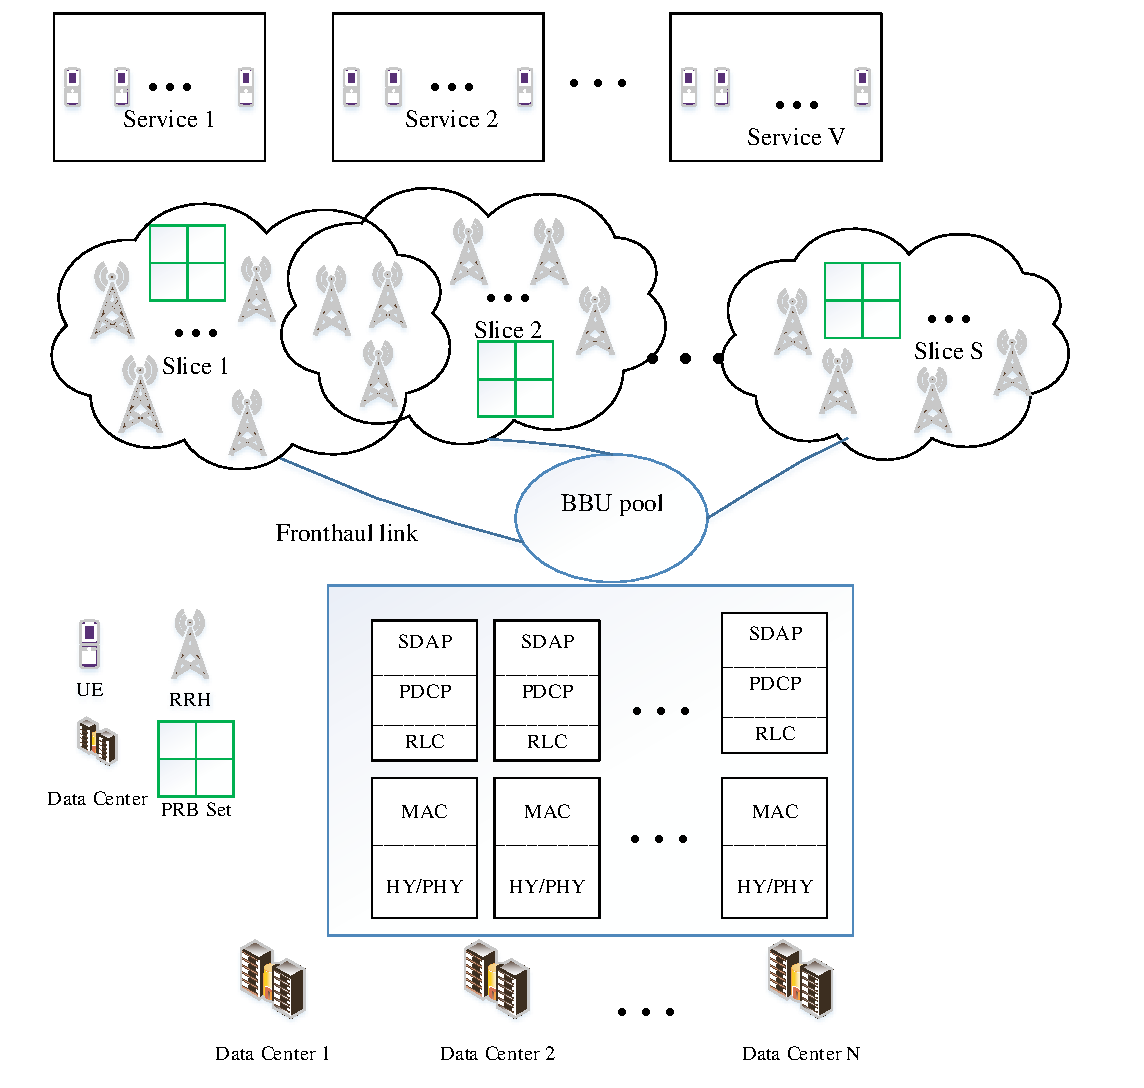
\includegraphics[scale=0.55]{c5}
  \caption{Network sliced O-RAN system}
  \label{fig:c11}
\end{figure} 
To evolve servicing in 5G, separation of elements of software and hardware of network is deployed in network functions virtualization (NFV) technology. In this technology, the functionality of networks is virtualized and divided into blocks of virtual network function (VNF).
The responsibility of wireless systems of the fifth generation covers wide range types of services. In order to provide the requirements of these services, NS is implemented to virtualize the shared physical network into several logical end-to-end networks. Three different types of NS are introduced in \cite{ns1} contains Core Slicing, RAN Slicing and Core-RAN Slicing. In Core-RAN Slicing, each slice of RAN is mapped to slices of Core. Also, UEs classified into a group of services according to their requirements. In addition, each service is connected to one or more Core-RAN slices based on the resource of slices.
Using cloud-computing in BBU-Pool, the performance of the system is enhanced by virtualizing resources
into virtual machines (VMs).
Each VM has a computing processor in order to be run by the Virtual Network Functions (VNFs) which processed arrival data. Also, VNFs are mapped to physical resources through NS techniques\cite{frdl,luong2018novel,luong2018novel1}. 


The compression of messages passed through the fronthaul link due to the limited capacity of these links is considered in \cite{simeone2016cloud,1111}. 
In \cite{lee2018dynamic}, dynamic network slicing is considered in Heterogeneous CRAN (H-CRAN) to maximize the weighted sum rate. Moreover, in \cite{frdl,luong2018novel,luong2018novel1} minimization of cost obtained by power consumption, also cloud processing and limited fronthaul capacity is considered. Furthermore, processing delay of each VM and wireless transmission delay is bounded.

 
In this paper, as  depicted in figure \ref{fig:c11}, the downlink of the O-RAN system is assumed. UEs are divided to different groups according to 
their service requirements. Also RAN is decoupled to slices to provide requirements of services. Optimal power allocation and joint connecting slices to services are applied. In addition, connecting slices to physical resources is taken to account.


\section{System Model and Problem Formulation}
In this section, first, we present the downlink (DL) of the O-RAN System. Then we obtain achievable rates and delays.
Afterward, the main problem is expressed.
\subsection{System Model}
Suppose there are $S$ slices Serving $V$ services. Each Service $v\in \{1,2,...,V \} $, consists of $U_v$ single-antenna user equipments (UEs) that require certain service. Each slice $s \in \{1,2,...,S \}$ consists of $R_s$ RRHs and $K_s$ Physical Resource Blocks (PRBs) as it is defined in the standard of LTE that the bandwidth (BW) of the channel is divided to PRBs in time series \cite{lee2018dynamic}. All RRHs in a slice that is connected to a service, transmit signals cooperatively to all the UEs in specific service \cite{motalleb2017optimal,mimoCran}. Each RRH $r \in \{1,2,...,R \}$ is connected to BBU pool via an optical fiber link with limited fronthaul capacity.
Suppose we have two processing layers in the BBU-Pool of O-RAN system. The lower layer is consist of high-PHY and MAC, and the upper layer is consist of RLC, PDCP and SDAP.
Assume we have $M_1$ VMs in the first layer and $M_2$ VMs in the second layer for processing data .
For simplicity, suppose each VNF run on a VM and there is a one-to-one connection between VNFs and VMs.
Each VNF in both layers connects to one or more slices. So in $s^{th}$ slice, there are $M_{s_1}$ VNFs in the first layer and $M_{s_2}$ VNFs in the second layer. All VNFs in first and second layer has the computational capacity that is  equal to $\mu_1$ and $\mu_2$, respectively. 
Also, RRHs and PRBs can serve more than one slices. 
\subsection{Achievable Rate}
The achievable data rate for $i^{th}$ UE in $v^{th}$ service can be written as 
\begin{equation}\label{eq1}
\mathcal{R}_{u(v,i)} = B \log_2({1+ \rho_{u(v,i)}});
\end{equation}
Where $B$ is the bandwidth of system and $\rho_{u(v,i)}$ is the SNR of $i^{th}$ UE in $v^{th}$ service which is obtained from 
\begin{equation}\label{eq2}
\rho_{u(v,i)} =  \frac{p_{u(v,i)}\sum_{s=1}^{S}|\bold{h}_{R_s,u(v,i)}^H \bold{w}_{R_s,u(v,i)}|^2 a_{v,s}}{BN_0 + I_{u(v,i)}};
\end{equation}
Where $p_{u(v,i)}$ represents the transmission power allocated by RRHs to $i^{th}$ UE in $v^{th}$ service, also, 
$\bold{h}_{R_s,u(v,i)} \in \mathbb{C}^{{R}_s}$ is the vector of channel gain of a wireless link from RRHs in the $s^{th}$ slice to the $i^{th}$ UE in $v^{th}$ service. In addition, $\bold{w}_{R_s,u(v,i)} \in \mathbb{C}^{{R}_s}$ depicts the  transmit beamforming vector from RRHs in the $s^{th}$ slice to the $i^{th}$ UE in $v^{th}$ service. Moreover, $BN_0$ denotes the power of Gaussian additive noise, and $I_{u(v,i)}$ is the power of interfering signals. Moreover, $a_{v,s} \in \{0,1\}$ is a binary variable that illustrates whether slice $s$ is connected to service $v$ or not. If $a_{v,s} =1$ then, $v^{th}$ service is connected to $s^{th}$ slice; otherwise, it is not connected.
\newline 
To obtain SNR as formulated in \eqref{eq2}, let $\bold{y}_{U_v}\in \mathbb{C}^{U_v} $ be the received signal's vector of all users in $v^{th}$ service which is given by \eqref{eq3}
\begin{equation}\label{eq3}
\bold{y}_{U_v} = \sum_{s = 1}^{S}\sum_{k=1}^{K_s} \boldsymbol{H}^H_{\mathcal{R}_s,\mathcal{U}_v}(\boldsymbol{W}_{\mathcal{R}_s,\mathcal{U}_v}\boldsymbol{P}_{U_v}^{\frac{1}{2}}\boldsymbol{x}_{\mathcal{U}_v}+ \boldsymbol{q}_{R_s}) \zeta_{U_v,k,s} a_{v,s}+ \boldsymbol{z}_{\mathcal{U}_v};
\end{equation}
Where $\boldsymbol{x}_{ \mathcal{U}_v} = [x_{ u_{(v,1)}},...,x_{ u_{(v,\mathcal{U}_v)}}]^T \in \mathbb{C}^{{R}_s } $ depicts the transmitted symbol vector of UEs in $v^{th}$ set of service,  $\boldsymbol{z}_{U_v}$ is the additive Gaussian noise $\boldsymbol{z_{U_v}} \backsim \mathcal{N}(0,N_0\boldsymbol{I}_{{U}_v})$ and $N_0$ is the noise power.
In addition, $\boldsymbol{q}_{R_s} \in \mathbb{C}^{{R}_s }  $ indicates the quantization noise which, is made from signal compression in BBU.
Besides, $\boldsymbol{P}_{U_v} = diag(p_{u_{(v,1)}}, ..., p_{u_{(v,\mathcal{U}_v)}})$.
\newline
Furthermore, $\zeta_{U_v,k,s} \delequal \{\zeta_{u(v,1),k,s},\zeta_{u(v,2),k,s},...,\zeta_{u(v,N_{U_v}),k,s}\}$,
$\zeta_{u(v,i),k,s} \in \{0,1\}$ is a binary parameter, demonstrates whether $i^{th}$ UE in $v^{th}$ service can transmit its signals through $k^{th}$ PRB and also this PRB belongs to $s^{th}$ slice or not.
$\boldsymbol{H}_{\mathcal{R}_s,\mathcal{U}_v}=\left[\boldsymbol{h}_{\mathcal{R}_s,u_{(v,1)}},\ldots,\boldsymbol{h}_{\mathcal{R}_s,v_{(v,\mathcal{U}_v)}}\right]^T  \in \mathbb{C}^{{R}_s\times {U}_v }$ 
shows the channel matrix between RRH set $\mathcal{R}_s$ to UE set
$\mathcal{U}_v$, besides. 
%The channel vector from the RRH of  $s^{th}$ slice to the $i^{th}$ UE in the $v^{th}$ service $\boldsymbol{h}_{\mathcal{R}_s,u_{(v,i)}}\in \mathbb{C}^{{R}_s}$ is modeled as below
%\begin{equation}
%\boldsymbol{h}_{\mathcal{R}_s,u_{(s,i)}} = \boldsymbol{\beta}^\frac{1}{2}_{\mathcal{R}_s,u_{(v,i)}} \boldsymbol{g}_{\mathcal{R}_s,u_{(v,i)}},
%\end{equation}
%where $\boldsymbol{g}_{\mathcal{R}_s,u_{(v,i)}} \backsim \mathcal{N}(0,N_0\boldsymbol{I}_{\mathcal{U}_v})$ indicates the fast fading and flat fading channel vector and $\boldsymbol{\beta}_{\mathcal{R}_s,u_{(v,i)}}=\text{diag}(b_{r_{(s,1),u_{(v,i)}}},\ldots,b_{r_{(s,\mathcal{R}_s),u_{(v,i)}}})$
%represents the large scale fading matrix.
What's more, it is assumed we have perfect channel state information (CSI).\newline
Moreover, $\boldsymbol{W}_{\mathcal{R}_s,\mathcal{U}_v} = [\boldsymbol{w}_{\mathcal{R}_s,u(v,1)},...,\boldsymbol{w}_{\mathcal{R}_s,u(v,U_v)}] \in \mathbb{C}^{{R}_s\times U_v} $ is the zero forcing beamforming vector to minimize the interference which is indicated as below
\begin{equation}
\boldsymbol{W}_{\mathcal{R}_s,\mathcal{U}_v} = \boldsymbol{H}_{\mathcal{R}_s,\mathcal{U}_v}(\boldsymbol{H}_{\mathcal{R}_s,\mathcal{U}_v}^H \boldsymbol{H}_{\mathcal{R}_s,\mathcal{U}_v})^{-1}.
\end{equation}
Hence, the interference power of $i^{th}$ UE in $v^{th}$ service can be represented as follow
\begin{equation}
\begin{split}
 I_{u_{(v,i)}} &= 
 \underbrace{\sum_{s=1}^{S}\sum_{n=1}^{S}\sum_{\substack{l=1 \\ l\neq i}}^{{U}_v} \gamma_{1}  p_{u_{(v,l)}}a_{v,s}\zeta_{u_(v,i),n,s}\zeta_{u_(v,l),n,s}}_{\text{(intra-service interference)}}\\
&+ \underbrace{\sum_{\substack{y=1 \\ l\neq v}}^{V}\sum_{s=1}^{S}\sum_{n=1}^{S}\sum_{l=1}^{{U}_y} \gamma_{2}  p_{u_{(y,l)}}a_{y,s} \zeta_{u_(v,i),n,s}\zeta_{u_(y,l),n,s}}_{\text{(inter-service interference)}}\\
&+\underbrace{ \sum_{s=1}^{S} \sum_{j=1}^{{R}_s} {\sigma_q}_{r_{(s,j)}}^2 |\boldsymbol{h}_{r_{(s,j)}, u_{(v,i)}}|^2 a_{v,s}}_{\text{(quantization noise interference)}}.
\end{split}
\end{equation}
Where, $\gamma_{1} =|\boldsymbol{h}_{\mathcal{R}_s, u_{(v,i)}}^H \boldsymbol{w}_{\mathcal{R}_{s},u_{(v,l)}}|^2$
and $\gamma_{2} =|\boldsymbol{h}_{\mathcal{R}_s, u_{(v,i)}}^H \boldsymbol{w}_{\mathcal{R}_{s},u_{(y,l)}}|^2$. Moreover,
${\sigma_q}_{r_{(s,j)}}$ is the variance of quantization noise of $j^{th}$ RRH in $s^{th}$ slice.
As it is clear, Interference signal for each UE is comming from UEs using the same PRB.
If we replace $p_{u_{(v,l)}}$ and $p_{u_{(y,l)}}$ by $P_{max}$, an upper bound $\bar{I}_{u_{(v,i)}}$ is obtained for $I_{u_{(v,i)}}$. Therefore, $\bar{\mathcal{R}}_{u_{(v,i)}} \forall v , \forall i$ is derived by using $\bar{I}_{u_{(v,i)}}$ instead of $I_{u_{(v,i)}}$ in  \eqref{eq1} and \eqref{eq2}.\newline
let $\bar{p}_{r_{(s,j)}}$ denote the power of transmitted signal from $j^{th}$ RRH in $s^{th}$ slice.
from \eqref{eq3} we have,
\begin{equation}
\bar{p}_{r_{(s,j)}} = \sum_{v=1}^{V}\boldsymbol{w}_{r_{(s,j)},\mathcal{U}_{v}} \boldsymbol{P}_{\mathcal{U}_v}^{\frac{1}{2}} \boldsymbol{P}_{\mathcal{U}_v}^{H \frac{1}{2}}   \boldsymbol{w}_{r_{(s,j)},\mathcal{U}_{v}}^H a_{v,s} + \sigma_{q_{r(s,j)}}^2.
\end{equation}
As a result the rate of users on the fronthual link between BBU-Pool and the $j^{th}$ RRH in $s^{th}$ slice is formulated as 
\begin{equation}
C_{R_{(s,j)}} = \log{(1+\sum_{v=1}^{V}\frac{w_{r_{(s,j)},\mathcal{D}_{s}} \boldsymbol{P}_{\mathcal{U}_v}^{\frac{1}{2}} \boldsymbol{P}_{\mathcal{U}_v}^{H \frac{1}{2}}   w_{r_{(s,j)},\mathcal{U}_{v}}^H a_{v,s}}{ \sigma_{q_{r(s,j)}}^2})},
\end{equation}
Where, $a_{v,s}$ is a binary variable denotes whether the slice $s$ is connected to service $v$ or not \cite{simeone2016cloud, 1111}.
\subsection{Mean Delay}
Let the packet arrival of UEs have a Poisson Process with arrival rate $\lambda_{u(v,i)}$ for $i^{th}$ UE of $v^{th}$ service. 
Therefore, the mean arrival data rate of UEs connect to $s^{th}$ slice in the first layer is 
$\alpha_{s_1} = \sum_{v=1}^{V}\sum_{u=2}^{U_v}a_{v,s}\lambda_{u(v,i)}$.  
Furthermore, the mean arrival data rate of the second layer is approximately equal to the mean arrival data rate of first layer $\alpha_{s} =\alpha_{s_1} \approx \alpha_{s_2}$ since, by using Burke’s Theorem, the mean arrival data rate of the second layer which is processed in the first layer is still Poisson with rate $\alpha_{s}$. 
It is assumed there are dispatchers in each layer for each slice to divide the incoming traffic to VNFs \cite{frdl,luong2018novel,luong2018novel1}.
Suppose the baseband processing of each VNF is depicted as a M/M/1 processing queue.
Each packet is routed by one of VNFs of slices. So the mean delay of slice $s$ which is related to incoming traffic rate routed to
each VNF in the first layer can be written as follow
\begin{equation}
d_{s_1} = \frac{1}{\mu_1 - \alpha_{s}/{M_{s_1}}}.
\end{equation}
Also, the delay of $s^{th}$ slice in the second layer is
\begin{equation}
d_{s_2} = \frac{1}{\mu_2 - \alpha_{s}/{M_{s_2}}}.
\end{equation}
In addition, $d_{s_{tr}}$ is the transmission delay for $s^{th}$ slice as a result of wireless transmission. The arrival data rate of wireless transmission
 is equal to the arrival data rate of dispatchers (used as a traffic divider) for each slice divide traffic data and transmit divided traffic to VNFs.
Moreover, it is assumed that the service time of transmission queue for each slice $s$ has 
 an exponential distribution with mean $1/(R_{{tot}_s})$ and can be modeled as a M/M/1 queue \cite{frdl,luong2018novel,luong2018novel1}. Therefore, 
the mean delay of the transmission layer is 
\begin{equation}
d_{s_{tr}} = \frac{1}{R_{{tot}_s} - \alpha_{s}};
\end{equation}
Where, $R_{{tot}_s} =  \sum_{v=1}^{V}\sum_{u=2}^{U_v}a_{v,s}R_{u(v,i)}$.
Mean delay of each slice is
\begin{equation}
D_{s} = d_{s_1} + d_{s_2} + d_{s_{tr}} \forall s.
\end{equation} 
\subsection{Physical Data Center Resource}
Each VNF requires
physical resources that contain RAM, Memory, and CPU.
Let, the required resources for VNF $f$ in slice $s$ is represented by a three-dimensional vector as follow
\begin{equation}
\bar{\Omega}_{(f,s)} = \{\Omega_{R_{f,s}}, \Omega_{M_{f,s}}, \Omega_{C_{f,s}} \};
\end{equation} 
Where,$\bar{\Omega}_{(f,s)}\in \mathbb{C}^{3}$ and $\Omega_{R_{f,s}}, \Omega_{M_{f,s}}, \Omega_{C_{f,s}}$ indicate the amount of required RAM, Memory, and CPU, respectively.
Moreover total amount of required RAM, Memory, and CPU of all VNFs of a slice is a three-dimensional vector which is defined as
\begin{equation}
\bar{\Omega}_{s}^{tot} = \sum_{f=1}^{M_{s_1} + M_{s_2}}\bar{\Omega}_{(f,s)};
\end{equation}
Also, there are $D_c$ data centers (DC), which served VNFs. Each DC contains several servers that supply VNF's requirements.
The amount of RAM, Memory, and CPU is denoted by $\tau_{R_{j}}, \tau_{M_{j}}$and $\tau_{C_{j}} $ for $j^{th}$ DC, respectively.
\begin{equation*}
\tau_j = \{\tau_{R_{j}}, \tau_{M_{j}}, \tau_{C_{j}} \};
\end{equation*}
Also we define a weighted parameter of $\tau_j$ as follow
\begin{equation}\label{wt}
\begin{split}
\hat{\Omega}_{s}^{tot} &= w_R \bar{\Omega}_{R_s}^{tot} + w_M \bar{\Omega}_{M_s}^{tot} + w_C \bar{\Omega}_{C_s}^{tot} \\
\hat{\tau}_j &= w_R \tau_{R_{j}} + w_M \tau_{M_{j}} + w_C \tau_{C_{j}},
\end{split}
\end{equation}
Where, $\boldsymbol{w} = \{w_R, w_M, w_C\}$ is the weight of RAM, Memory, and CPU that is used for Algorithm \ref{alg3}.
In this system model, the placement of physical DC resources to VNFs is considered. $y_{s,d}$ is a binary variable indicates whether $d^{th}$ DC is connected to VNFs of $s^{th}$ slice or not.
\subsection{Problem Statement}
One of the most important parameters to estimate the optimality of the system is energy efficiency which is represented as a sum-rate to sum-power 
\begin{equation}
\eta(\boldsymbol{P},\boldsymbol{A}) := \frac{\sum\limits_{v=1}^{V} \sum\limits_{k=1}^{{U}_v}\mathcal{R}_{u_{(v,k)}} }{\sum\limits_{s=1}^{S} \sum\limits_{i=1}^{{R}_s}\bar{p}_{r_{(s,i)}}} = \frac{\mathfrak{R}_{tot}(\boldsymbol{P},\boldsymbol{A})}{P_{r_{tot}}(\boldsymbol{P},\boldsymbol{A})},
\end{equation}
Where, $\sum\limits_{s=1}^{S}\sum\limits_{i=1}^{{R}_s}\bar{p}_{r_{(s,i)}}$ is the total power consumption of all RRHs in all slices. Also, $\sum\limits_{v=1}^{V} \sum\limits_{k=1}^{{U}_v}\mathcal{R}_{u_{(v,k)}} $ is the toal rates of all UEs applied for all types of services. 
Assume the power consumption of baseband processing at each DC $d$ that is connected to VNFs of a slice $s$ is depicted as
$\phi_{s,d}$. So the total power of the system for all active DCs that are connected to slices can be represented as  
\begin{equation*}
\phi_{tot} = \sum_{s=1}^{S}\sum_{d=1}^{D_c}y_{s,d}\phi_{s,d}.
\end{equation*} 
In this paper, the main goal is to maximize sum-rate and minimize sum-power (the total power of all RRHs and the total power consumption of baseband processing at all DCs) simultaneously, with the presence of constraints which is written as follow, 
\begin{subequations}
\begin{alignat}{4}
\max\limits_{\boldsymbol{P}, \boldsymbol{A}, \boldsymbol{Y} }   \quad &   \eta(\boldsymbol{P},\boldsymbol{A})+\frac{1}{\phi_{tot}(\boldsymbol{Y})} \\
\text{subject to} \quad  & \bar{p}_{r_{(s,i)}} \leq P_{max} && \quad \forall s, \forall i, 
 \label{c11} \\
&p_{u_{(v,k)}}  \geq 0  &&\quad \forall v, \forall k,\label{c12} \\
&\mathcal{R}_{u_{(v,k)}} \geq  \mathcal{R}_{u_{(v,k)}}^{min} && \quad \forall v, \forall k,\label{c13} \\                                 
&C_{r_{(s,i)}} \leq C_{r_{(s,i)}}^{max}  &&\quad \forall s, \forall i, \label{c14}\\
&D_{s} \leq D_{s}^{max}  &&\quad \forall s,\label{c15} \\
& \sum_{s=1}^{S}a_{v,s} \geq 1 &&\quad \forall s, \label{c21} \\
& \sum_{d=1}^{D_c}\sum_{v=1}^{V}y_{s,d}a_{v,s} \geq 1\times\sum_{v=1}^{V}a_{v,s} &&\quad \forall s,\label{c23} \\
& \bar{\Omega}_{\mathfrak{z}(s)}^{tot} = \sum_{f=1}^{F_s}\bar{\Omega}_{\mathfrak{z}(f,s)} \leq  \sum_{d=1}^{D_c} y_{s,d} \tau_{\mathfrak{z}_d}                      
 && \quad \forall \mathfrak{z}, \forall s; \label{c22}
\end{alignat}
\label{constraints}
\end{subequations}
Where,$\boldsymbol{P} =[p_{u(v,k)}]  \forall v , \forall k $, is the matrix of power for UEs, $\boldsymbol{A} =[a_{v,s}]  \forall v , \forall s $ denotes the binary variable for connecting slices to services and $\boldsymbol{Y} =[y_{s,d}]   \forall s ,  \forall d $ is a binary variable shown whether 
the physical DC is connected to a VNFs of a slice or not. 
\eqref{c11} and \eqref{c12} indicate that the power of each RRH do not exceed the maximum power, and the power of each UE is a positive integer value, respectively. Also \eqref{c13} shows that the rate of each UE is more than a threshold. \eqref{c14} and \eqref{c15} depicts that the capacity of the fronthaul link is limited, and the delay of receiving signal should be less than a threshold, respectively.  
Furthermore, \eqref{c21}
ensures that each service is connected to one or more slices.
Also, \eqref{c23} guarantees that each slice (VNFs in two layers of slices) has been placed to one or more physical resources of DCs. Moreover, \eqref{c22}  $\mathfrak{z}\in \{M,R,C\}$, supports 
that we have enough physical resources for VNFs of each slice.\newline 
The main optimizaiton problem which, is formulated as \eqref{constraints}, can be decomposed into two independent optimization problems A and B since the variables can be obtained independently. Problem A is defined as 
\begin{subequations}
\begin{alignat}{4}
\max\limits_{\boldsymbol{P}, \boldsymbol{A} }   \quad &   \eta(\boldsymbol{P},\boldsymbol{A})\\
\text{subject to} \quad  & \bar{p}_{r_{(s,i)}} \leq P_{max} && \quad \forall s, \forall i,   \\
&p_{u_{(v,k)}}  \geq 0  &&\quad \forall v, \forall k, \\
&\mathcal{R}_{u_{(v,k)}} \geq  \mathcal{R}_{u_{(v,k)}}^{min} && \quad \forall v, \forall k, \\                                 
&C_{r_{(s,i)}} \leq C_{r_{(s,i)}}^{max}  &&\quad \forall s, \forall i,\label{cc14} \\
&D_{s} \leq D_{s}^{max}  &&\quad \forall s, \label{cc15} \\
& \sum_{s=1}^{S}a_{v,s} \geq 1 &&\quad \forall s.
\end{alignat} 
\label{constraints1}
\end{subequations}
Problem B is 
\begin{subequations}
\begin{alignat}{4}
\min\limits_{\boldsymbol{y} }   \quad &   \phi_{tot}(\boldsymbol{Y})\\
\text{subject to} \quad & \sum_{d=1}^{D_c}\sum_{v=1}^{V}y_{s,d}a_{v,s} \geq 1\times\sum_{v=1}^{V}a_{v,s} &&\quad \forall s, \\
&  \bar{\Omega}_{\mathfrak{z}(s)}^{tot} = \sum_{f=1}^{F_s}\bar{\Omega}_{\mathfrak{z}(f,s)} \leq  \sum_{d=1}^{D_c} y_{s,d} \tau_{\mathfrak{z}_d}                      
 && \quad \forall \mathfrak{z}, \forall s. \label{eqomega}
\end{alignat}
\label{constraints2}
\end{subequations}
\section{Proposed Method For Problem \eqref{constraints1}}
In this subsection, the proposed method is applied to solve the optimization problem.
We want to solve \eqref{constraints1}. Since the problem is non-convex and NP-Hard, iterative algorithm is applied.
To solve the problem and obtain $\boldsymbol{A}$ and $\boldsymbol{P}$ we divide problem \eqref{constraints1} into 
two different part that can be solved iteratively.  
\subsection{First Part of Sub-Problem A}\label{firstsub}
Firstly, we need to obtain $\boldsymbol{A}$ by fixing $\boldsymbol{P}$ in the problem \eqref{constraints1} and updating this parameter at the end of each iteration. Two different methods are applied to acquire $\boldsymbol{A}$. 
The details of the heuristic algorithm are represented in \textbf{Algorithm} \eqref{alg}.  
\begin{algorithm}
\caption{Mapping Slice to Service}\label{alg}
\begin{algorithmic}[1]
\State Sort services according to the number of UEs in it and their requirements in the descending order.
\State Sort slices according to the weighted linear combination of number of PRBs, RRHs and VNFs in two layers and the Capacity of their resources in the descending order. 
\For {$i \gets 1$ to $S$}
\For {$j \gets 1$ to $V$}
\State Set $a_{i,j} = 1$
\State Obtain Parameters of Systems (power and rate of UEs, rate of fronhaul links, power of RRHs)
\If {conditions \eqref{c11}, \eqref{c12}, \eqref{c13} and \eqref{c14} is not applied} 
\State Set $a_{i,j} = 0$;
\Else
\State break from inner loop;
\EndIf 
\State \textbf{end if}
\EndFor 
\State \textbf{end for}
\EndFor 
\State \textbf{end for}
\end{algorithmic}
\end{algorithm}
\subsection{Second Part of Sub-Problem A}\label{secondsub}
In this part, by assuming that $\boldsymbol{A}$ is fixed, the power of UEs in each service is achieved.
\begin{theorem}\label{t2}
 $\eta^*$ which is the optimum energy efficiency can be achieved if
\begin{equation}\label{q2}
\begin{split}
&\max \limits_{\boldsymbol{P}} (\mathfrak{R}_{tot}(\boldsymbol{P}) - \eta^* P_{r_{tot}}(\boldsymbol{P}))=\\
& \mathfrak{R}_{tot}(\boldsymbol{P}^*) - \eta^* P_{r_{tot}}(\boldsymbol{P}^*) =0.
\end{split}
\end{equation}
\end{theorem}
\begin{proof}
See \cite{aaa}, Appendix A
\end{proof}
The second subproblem can  be solved using the Lagrangian function and iterative algorithm. 
Since, Interference is a function of the power of UEs, for simplicity, we assume an upper bound $\bar{I}_{u_{(v,i)}}$ for interference (the worst-case). 
In order to make \eqref{constraints1} as a standard form of a convex optimization problem, it is required to change the variable of equations \eqref{cc14} and \eqref{cc15}.
The Lagrangian function is written as follow
\begin{equation}\label{lagrang}
\begin{split}
\mathcal{L}(\boldsymbol{P}; \boldsymbol{\lambda}, \boldsymbol{\mu}, \boldsymbol{ \xi}, \boldsymbol{ \kappa}) & = \sum\limits_{v=1}^{V} \sum\limits_{k=1}^{U_v}\mathcal{\bar{R}}_{u_{(v,k)}} 
- \eta \sum\limits_{v=1}^{V} \sum\limits_{i=1}^{\mathcal{R}_s}\bar{p}_{r_{(s,i)}}\\
&+\sum\limits_{s=1}^{S} \sum\limits_{k=1}^{U_v} \lambda_{u_{(v,k)}} (\mathcal{\bar{R}}_{d_{(s,k)}}-\mathcal{R}_{u_{(v,k)}}^{max})\\
&- \sum\limits_{s=1}^{S} \sum\limits_{i=1}^{R_s} \mu_{r_{(s,i)}} (\bar{p}_{r_{(s,i)}}-P_{max})\\
&- \sum\limits_{s=1}^{S} \sum\limits_{i=1}^{R_s} \xi_{r_{(s,i)}} (\bar{p}_{r_{(s,i)}}-\sigma_{q_{r(s,j)}}^2 2^{C_{r_{(s,i)}}^{max}}).\\ 
&+ \sum\limits_{v=1}^{V} \sum\limits_{k=1}^{U_v} \kappa_{u_{(v,k)}} \sum\limits_{s=1}^{S}(R_{u_{(v,k)}} -\mathfrak{D_s})a_{v,s}.\\ 
\end{split}
\end{equation}
Where, $\mathfrak{D_s}=\frac{1}{D_{s}^{max}-d_{s_1}-d_{s_2}}+\alpha_s$. Also, $\boldsymbol{\lambda}$, $\boldsymbol{\mu}$, $\boldsymbol{\xi}$, and $\boldsymbol{ \kappa}$ are the matrix of Lagrangian multipliers that have non-zero positive elements. Optimal power is obtained from equation \eqref{lagrang} as follow
\begin{equation}
p_{u(v,i)}^{*} = [\frac{\mathfrak{y}_{u(v,i)}\mathfrak{w}_{u(v,i)}-\mathfrak{x}_{u(v,i)}\mathfrak{z}_{u(v,i)}}{\mathfrak{x}_{u(v,i)}\mathfrak{w}_{u(v,i)} }]^+
\end{equation}
where, $\mathfrak{y}_{u(v,i)}= (\lambda_{u(v,i)}+\kappa_{u_{(v,k)}}+1)\frac{B}{Ln_2}$ and 
$\mathfrak{w}_{u(v,i)} = \sum_{s=1}^{S}|\bold{h}_{R_s,u(v,i)}^H \bold{w}_{R_s,u(v,i)}|^2 a_{v,s}$. Also 
$\mathfrak{z}_{u(v,i)} = BN_0 + \bar{I}_{u(v,i)}$ and $\mathfrak{x}_{u(v,i)} = \sum\limits_{s=1}^{S} \sum\limits_{i=1}^{R_s} ( \mu_{r_{u(s,i)}} + \xi_{r_{(s,i)}}+\eta)||w_{r_{(s,j)},u_{(v,i)}}||^2$. 
By using sub-gradient method, the optimal power $\boldsymbol{P}$ is obtained. 
%\section*{References}
\subsection{Solving two part of Sub-problem A iteratively}
In \eqref{firstsub} and \eqref{secondsub}, the details of solving each part of the subproblem are depicted. 
Firstly, by the fixing power of each UE, $\boldsymbol{A}$ is obtained using Algorithm \eqref{alg}. Then by using the sub-gradient method, \eqref{secondsub} is solved and iteratively solves these problems until variables converge.
Here, the algorithm of solving sub-problem A is shown in \textbf{Algorithm} \eqref{alg2}
\begin{algorithm}
\caption{Joint Network Slicing and Power Allocation}\label{alg2}
\begin{algorithmic}[1]
\State Set the maximum number of iterations $I_{max}$, convergence condition $\epsilon_{\eta}$  and the initial value $\eta^{(1)} = 0$
\State Set $\boldsymbol{P} = \boldsymbol{P}_{max}$
\For {$counter \gets 1$ to $I_{max}$}
\State Achieve $\boldsymbol{A}$ by applying Algorithm \eqref{alg}
\State Obtain $\boldsymbol{P}$ by using sub-gradient method which is mentioned in \eqref{secondsub}.
\If {$ \mathfrak{R}_{tot}(\boldsymbol{P}^{(i)},\boldsymbol{A}^{(i)}) - \eta^{(i)} P_{r_{tot}}(\boldsymbol{P}^{(i)},\boldsymbol{A}^{(i)}) < \epsilon_{\eta} $} 
\State Set $\boldsymbol{P}^*= \boldsymbol{P}^{(i)} $, $\boldsymbol{A}^*= \boldsymbol{A}^{(i)} $   and  $ \eta^{*} =\eta^{(i)} $;
\State break;
\Else
\State $i= i+1$, Setting $\boldsymbol{P} = \boldsymbol{P}^{(i)}$ ;
\EndIf 
\State \textbf{end if}
\EndFor 
\State \textbf{end for}
\end{algorithmic}
\end{algorithm}
\subsection{Sub-Problem B}
In this subsection, we want to solve  \eqref{constraints2}, which is the placement of virtual resources to physical resources in order to minimize the number of using DCs. 
To achieve optimum $\boldsymbol{Y}$ heuristic algorithm is applied. The details of the heuristic algorithm are written in \textbf{Algorithm} \eqref{alg3}. In this algorithm, firstly, we sort slices and DCs according to their sum weighted of their requirements. Secondly, we start mapping from the most needed slices to the DC with the most physical resources. After mapping DCs to slices, if some slices are not admitted, we start admitting remaining slices to more than one DCs. In the end, if DC with the lowest physical resources is free and can be served instead of DC with the highest physical resource, the slices remapped to new DC with the lowest physical resource since it has the lowest power consumption.  
If a slice does not admit to a specific DC, it remains for the next placement. In next placement the remaining slices, map to more than one DC according to their requirements.
\begin{algorithm}
\caption{Plecement of Physical resources into Virtual resources}\label{alg3}
\begin{algorithmic}[1]
\State Sort Slices according to $\hat{\Omega}_{s}^{tot} , \forall s$ in descending order.
\State Sort DCs according to $\hat{\tau}_j , \forall j$ in descending order. 
\State $\boldsymbol{Y} = \boldsymbol{0}$
\For {$d \gets 1$ to $D_c$}
\For {$s \gets 1$ to $S$}
\If {$\sum_{d=1}^{D_c}y_{s,d}==0$ and $\bar{\Omega}_{\mathfrak{z}(s)}^{tot} \leq \tau_{\mathfrak{z}_j} \forall \mathfrak{z}, \forall s$  } 
\State Set $y_{s,d} = 1$;
\State {$\tau_j$ $\gets$ {$\tau_j - \bar{\Omega}_{s}^{tot}$}}
\EndIf 
\State \textbf{end if}
\EndFor 
\State \textbf{end for}
\EndFor 
\State \textbf{end for}
\State  $\{ind_{remaining} = s|({\sum_{d=1}^{D_c}y_{s,d}==0})\}$
\State Sort remaining amount of DCs same as before in descending order.
\State Sort remaining slices same as before in descending order.
\For {$r \gets 1$ to $S_{remaining}$}
\For {$n \gets 1$ to $D_c$}
\State Set $y_{s,d} = 1$;
\State {$\bar{\Omega}_{s}^{tot}$ $\gets$ {$\bar{\Omega}_{s}^{tot}- \tau_j$}}
\If {$\bar{\Omega}_{s}^{tot}==0$}
\State Set $y_{s,d} = 1$;
\State {$\tau_j$ $\gets$ {$\tau_j - \bar{\Omega}_{s}^{tot}$}}
\State {break inner loop}
\EndIf 
\State \textbf{end if}
\EndFor 
\State \textbf{end for}
\EndFor 
\State \textbf{end for}
\State Remapping DCs must be done to prevent wasting Energy
\end{algorithmic}
\end{algorithm}
\section{Simulation}
In this section, simulation and numerical results for the main problem are depicted.
 \begin{table}
 \caption {Simulation Parameter} \label{table:1a} 
 \begin{center}
  \begin{tabular}{||c c ||} 
  \hline
Parameter & Value \\ [0.5ex] 
  \hline\hline
  Noise power & -174dBm\\
  \hline
  Bandwidth & 120 KHZ \\
  \hline
 Maxmimun transmit Power of each RRH & 40dBm \\
  \hline
   Maxmimun transmit Power of each UE & 30dBm \\
  \hline
  Minimum delay &  300usec \\
  \hline
  Maximum fronthaul capacity  & 20bits/sec/Hz \\ 
   \hline
  Minimum data rate &  120 kbits/sec \\ [1ex] 
  \hline
 \end{tabular}
 \end{center}
 \end{table}
In Fig. \ref{fig:f1a}, energy efficiency is depicted for two different numbers of services with the different mean number of UEs in each service (the parameters for simulation listed in table \ref{table:1a}). The optimal method is $0.016$ bits/J/Hz better than the proposed method for $V = 6$ and $E[U_v] = 10$, and also, $0.011$ bits/J/Hz better than the proposed method for $V = 3$ and, $E[U_v] = 10$. As it is shown, the Energy Efficiency is increased as a mean number of UEs rises.
\begin{figure}%[H]
  \centering
    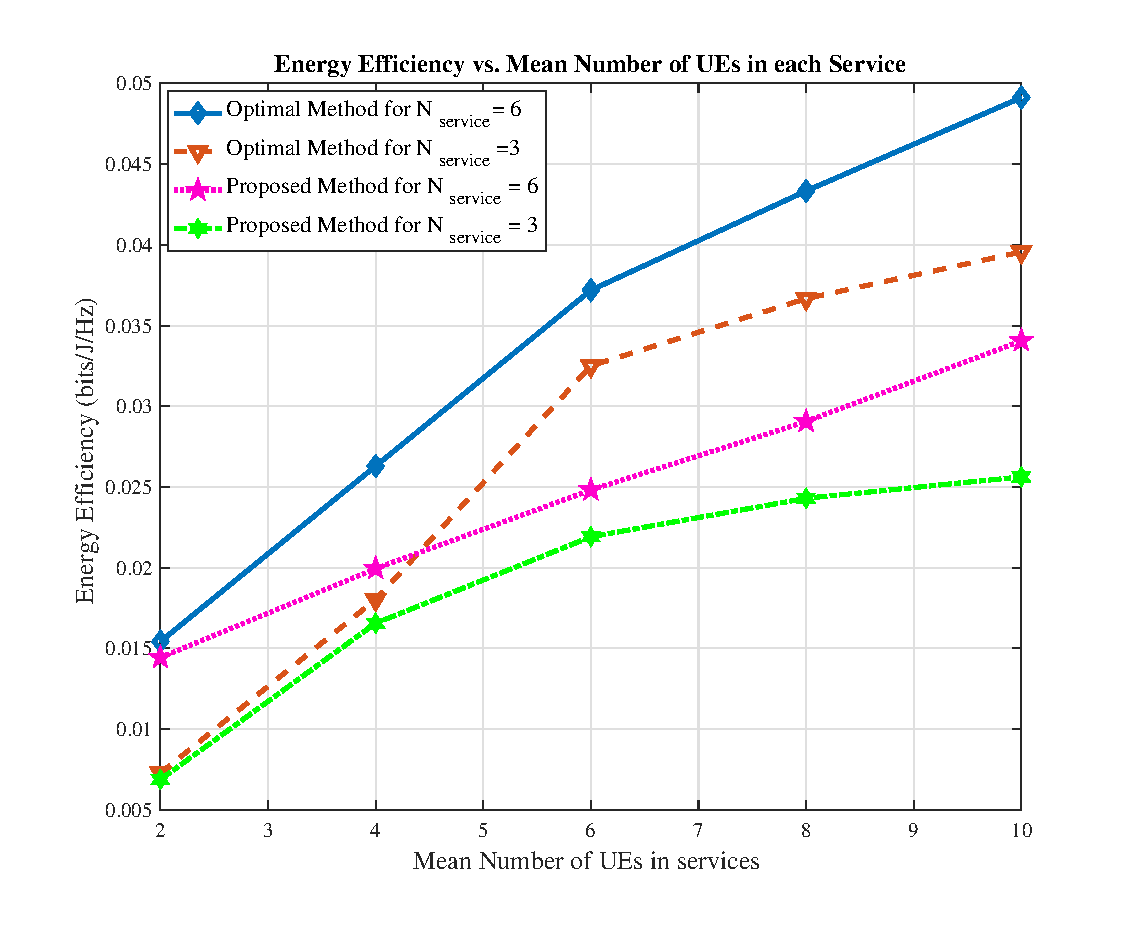
\includegraphics[width=\linewidth]{figure11}
  \caption{Energy Efficiency vs. Mean Number of UEs in each Service}
  \label{fig:f1a}
\end{figure} 
In Fig. \ref{fig:f1}, the ratio of admitted slices is demonstrated for two different numbers of DCs with the different number of slices (the parameters for simulation listed in table \ref{table:1} and \ref{table:2}). In this simulation, it is assumed that  just one DC can serve each slice, and it is not admitted by more than one DC. The proposed method is based on Algorithm \ref{alg3}, and the optimal method is done by the MOSEK toolbox.
 \begin{table}
 \caption {Simulation Parameter} \label{table:1} 
 \begin{center}
  \begin{tabular}{||c c ||} 
  \hline
  Parameter & Value \\ [0.5ex] 
  \hline\hline
  Mean of CPU for DCs & 25.6GHz\\
  \hline
  Mean of RAM for DCs & 128G\\
  \hline
 Mean of Memory for DCs & 10T \\
  \hline
   Mean of CPU for Slices & 3.2GHz\\
  \hline
  Mean of RAM for Slices & 16G\\
  \hline
 Mean of Memory for Slices & 1T \\ [1ex] 
  \hline
 \end{tabular}
 \end{center}
 \end{table}
When we have two DCs, the proposed method and optimal method have approximately the same ratio of admitted slices. But by increasing the number of DCs to five, the performance of the proposed method reduced. Using five DCs, the difference between the
proposed method and the optimal method in the worst case (44 slices) is about $23$ percentage. 
 \begin{table}
 \caption {Simulation Parameter} \label{table:2} 
 \begin{center}
  \begin{tabular}{||c c ||} 
  \hline
  Parameter & Value \\ [0.5ex] 
  \hline\hline
   $w_C$ & 320\\
  \hline
  $w_R$  & 64\\
  \hline
 $w_M$  & 1 \\ [1ex] 
  \hline
 \end{tabular}
 \end{center}
 \end{table}
\begin{figure}%[H]
  \centering
    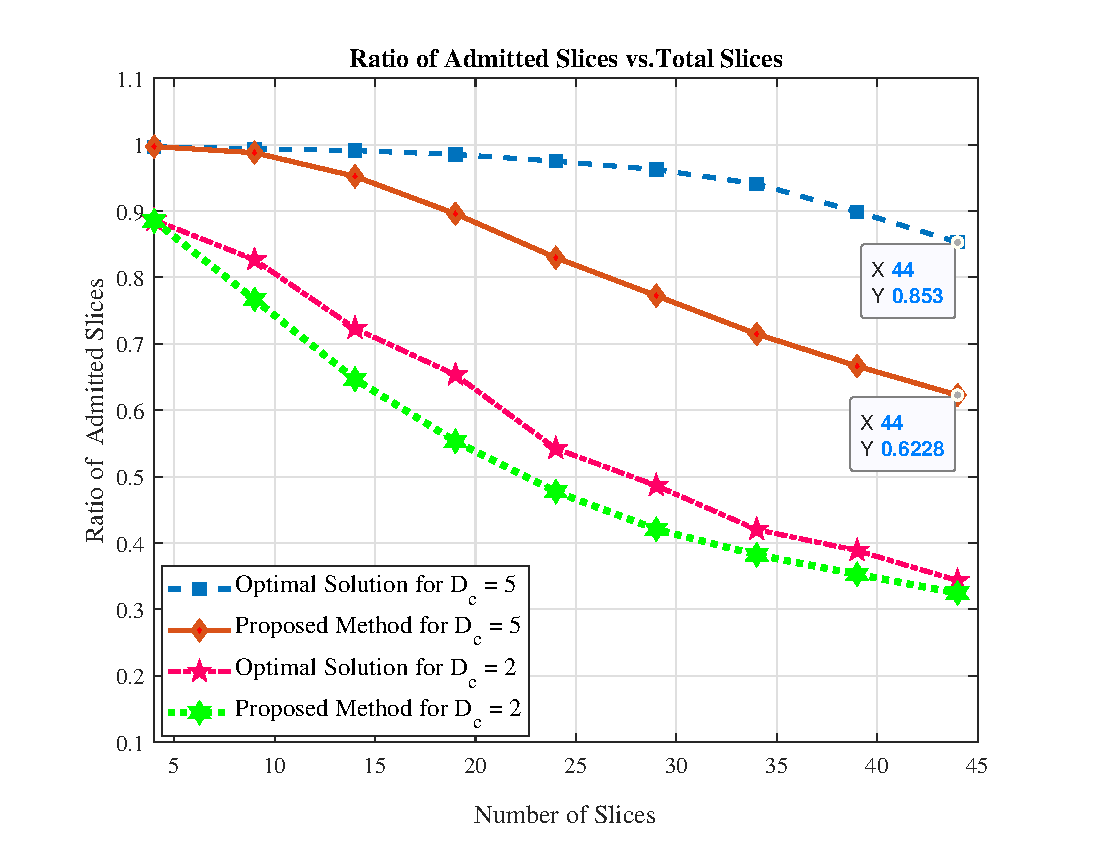
\includegraphics[width=\linewidth]{f111}
  \caption{Ratio of Admitted Slices connected to just one DC vs. Total slices}
  \label{fig:f1}
\end{figure} 
In Fig. \ref{fig:f2}, the normalized resource consumption is depicted due to the number of slices (the parameters for simulation listed in table \ref{table:1} and \ref{table:2}). In this simulation, it is assumed that the number of DCs is entirely enough to cover all slices. The optimality of the placement of DCs to slices is measured. It is shown that how much resources of active DCs are not used. For ten slices, the difference between the optimal solution and the proposed solution is about $15$ percent. 
\begin{figure}%[H]
  \centering
    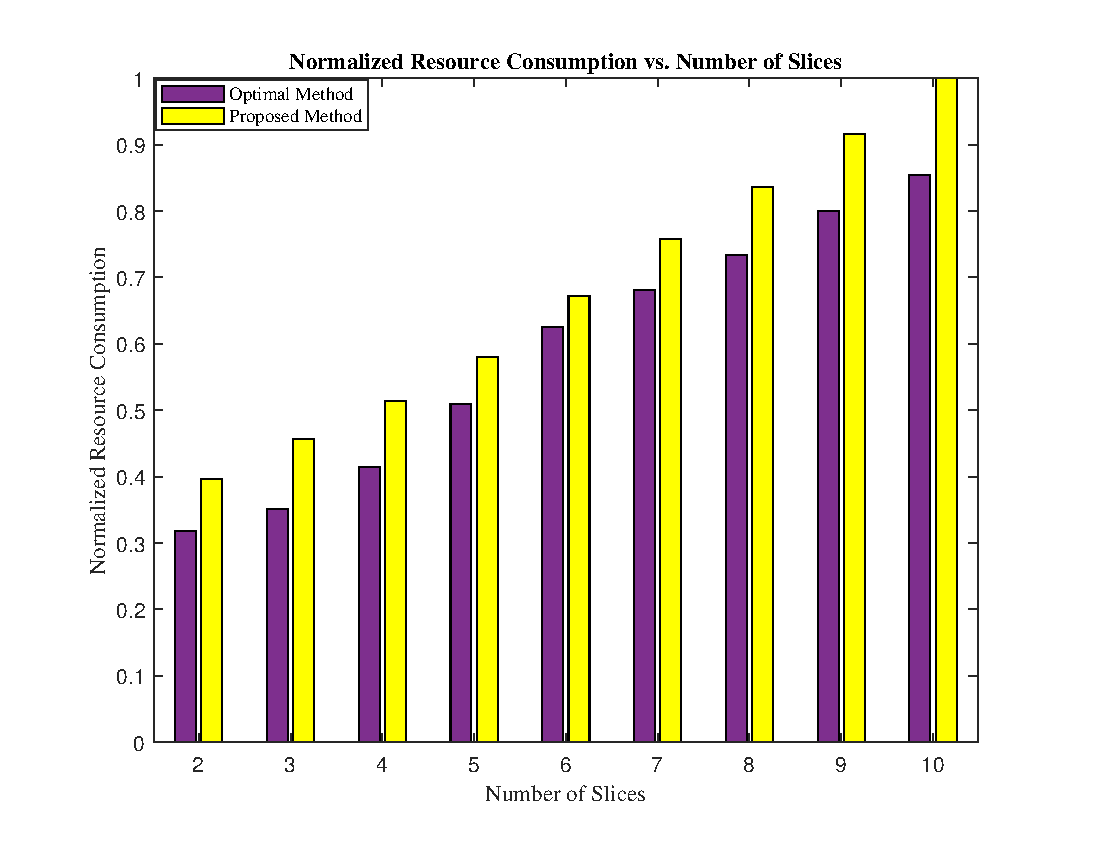
\includegraphics[width=\linewidth]{fig2_last}
  \caption{Normalized Resource Consumption vs. Number of Slices}
  \label{fig:f2}
\end{figure} 
\section{Conclusion}
In this paper, joint network slicing and power allocation is considered in an end to end O-RAN system.
It is assumed that UEs are classified based on their service requirements. Also, there is a number of slices served the services. Each slice, is consist of PRBs, RRHs, and VNFs that run on VMs. The limited fronthaul capacity is considered for the fiber links between RRHs and BBU-pool.
The target is to maximize the sum-rate and minimize the power consumption and energy cost of data centers simultaneously.
The problem is decomposed into two sub-problems. Each sub-problems are solved separately by a heuristic algorithm. For the sub-problem A, energy efficiency vs. mean number of UEs in each service is depicted. The energy efficiency  exceeded by increasing the mean number of UEs in each service. For the sub-problem B, two figures are shown. In the first one, the ratio of admitted slices that connect to just one DC, for a different number of slices is denoted. In the second figure, the normalized resource consumption of DCs is depicted. In each figure, the heuristic algorithm is compared with the optimal method and the difference between them is discussed.

 
\bibliographystyle{IEEEtran}
\bibliography{ref}
\end{document}
